%
\documentclass[final]{beamer} 
  \mode<presentation> {  
    \usetheme{Yale} 
  }

\definecolor{beamer@blendedblue}{HTML}{BD5319}
\usepackage{verbatim,bm}
\DeclareMathOperator*{\supp}{supp}
\DeclareMathOperator*{\diam}{diam}
\usepackage{tikz,fp}
\usetikzlibrary{calc,patterns}
  \usepackage[english]{babel}
%
  \usepackage{amsmath,amsthm, amssymb, latexsym}
  \usepackage[ruled,linesnumbered,vlined]{algorithm2e}
  \usepackage{bm}
  \usepackage{tcolorbox}
\usepackage{tabularx}
\usepackage{array}
\usepackage{colortbl}
\usepackage{cleveref}
\usepackage{algorithmicx}
\usepackage{algpseudocode}
\tcbuselibrary{skins}


\definecolor{YaleLightBlue}{HTML}{63AAFF}
\definecolor{YaleCoreBlue}{HTML}{00356B}
\definecolor{YaleDarkBlue}{HTML}{286DC0}
\definecolor{YaleLighterGrey}{HTML}{DDDDDD}
\definecolor{YaleLightGrey}{HTML}{978D85}
\definecolor{YaleCoreGrey}{HTML}{4A4A4A}
\definecolor{YaleDarkGrey}{HTML}{222222}
\definecolor{YaleCoreOrange}{HTML}{BD5319}
\definecolor{YaleCoreGreen}{HTML}{5F712D}
\definecolor{YaleGreen}{HTML}{5F712D}
\definecolor{DarkRed}{HTML}{B8433B}
\setbeamertemplate{caption}{\raggedright\insertcaption\par}
\setbeamercolor{caption}{fg=YaleCoreGreen}
\setlength\abovecaptionskip{-20pt}

\tcbset{tab2/.style={enhanced,fonttitle=\bfseries,fontupper=\normalsize\sffamily,
colback=YaleLightBlue!10!white,colframe=YaleCoreBlue,colbacktitle=YaleCoreBlue,
coltitle=black,center title}}




\newcommand{\Acc}{\text{Acc.}}
\newcommand{\Dis}{\text{G}_{\text{Discr.}}}
\newcommand{\LDis}{\text{L}_{\text{Discr.}}}
\newcommand{\Knn}{\text{kNN-Pred}}
\newcommand{\spaceClass}{\mathcal{H}}
\newcommand{\optimal}{h^*}
\newcommand{\optimalfair}{h^{*}_{\textup{fair}}}
\newcommand{\kr}{Kre\u{\i}n\xspace}

\DeclareMathOperator*{\essinf}{ess\,inf}
\DeclareMathOperator*{\esssup}{ess\,sup}
\DeclareMathOperator{\hel}{hel}
\DeclareMathOperator{\pr}{Pr}

\DeclareMathOperator{\sech}{sech}
\DeclareMathOperator{\csch}{csch}
\DeclareMathOperator{\mil}{mil}
\DeclareMathOperator{\sign}{sign}

\newcommand{\kl}[2]{D_{\mathrm{KL}}( #1 \parallel #2 )}
\newcommand{\js}[2]{D_{\mathrm{JS}}( #1 \parallel #2 )}
\newcommand{\wjs}[3]{D_{\mathrm{GJS}}^{#1}( #2 \parallel #3 )}
%\newcommand{\mil}[2]{D_{\mathrm{MIL}}( #1 \parallel #2 )}
\newcommand{\td}[2]{ \Delta ( #1 \parallel #2 )}


  %
  \usepackage{wrapfig}
  \usefonttheme[onlymath]{serif}
  \usepackage{graphicx}
  \boldmath
\usepackage[size=custom,width=152.4,height=91.44,scale=1.4,orientation=landskape]{beamerposter} 
\title{Locality-Sensitive Hashing for $f$-Divergences and \kr Kernels: 
	Mutual 
	Information Loss and Beyond}
\author{Lin Chen\inst{1,2}, 
	Hossein Esfandiari\inst{1},
	Thomas Fu\inst{1}, and
	Vahab Mirrokni\inst{1}
	 \vspace{10pt}}
\institute{{  \inst{1}Google Research, \inst{2}Yale University }\vspace{10pt}}
%

\newlength{\columnheight}
%
\setlength{\columnheight}{105cm}
%

\usepackage{forloop}
%\newcommand{\defcal}[1]{\expandafter\newcommand\csname 
%c#1\endcsname{{\mathcal{#1}}}}
%\newcommand{\defbb}[1]{\expandafter\newcommand\csname 
%b#1\endcsname{{\mathbb{#1}}}}
%\newcounter{calBbCounter}
%\forLoop{1}{26}{calBbCounter}{
%	\edef\letter{\Alph{calBbCounter}}
%	\expandafter\defcal\letter
%	\expandafter\defbb\letter
%}

% Caligraphics and Board Letters
\newcommand{\defcal}[1]{\expandafter\newcommand\csname 
	c#1\endcsname{{\mathcal{#1}}}}
\newcommand{\defbb}[1]{\expandafter\newcommand\csname 
	b#1\endcsname{{\mathbb{#1}}}}
\newcommand{\defbf}[1]{\expandafter\newcommand\csname 
	bf#1\endcsname{{\mathbf{#1}}}}
\newcounter{calBbCounter}
\forLoop{1}{26}{calBbCounter}{
	\edef\letter{\Alph{calBbCounter}}
	\expandafter\defcal\letter
	\expandafter\defbb\letter
	\expandafter\defbf\letter
}
\forLoop{1}{26}{calBbCounter}{
	\edef\letter{\alph{calBbCounter}}
	% 	\expandafter\defcal\letter
	% 	\expandafter\defbb\letter
	\expandafter\defbf\letter
}


\usepackage[absolute,overlay]{textpos}
%
\renewcommand{\vec}[1]{\mathbf{#1}}

\usepackage{nicefrac}       %
 
%
\PassOptionsToPackage{table,pdftex,dvipsnames}{xcolor}
\usepackage{array,booktabs,tabularx}
\usepackage{multirow}
\usepackage[numbers]{natbib}
\usepackage{subfigure}
\newcommand{\matroid}{\mathcal{I}}
\DeclareMathOperator{\round}{round}
\newcommand{\one}{\mathbf{1}}
\newcommand{\constraint}{\mathcal{K}}
\newcommand{\ie}{\emph{i.e.}\xspace}
\newcommand{\eg}{\emph{e.g.}\xspace}

\newcommand{\AlgMeta}{\texttt{Meta-Frank-Wolfe}\xspace}
\newcommand{\AlgVR}{\texttt{VR-Frank-Wolfe}\xspace}
\newcommand{\Alg}{\texttt{Mono-Frank-Wolfe}\xspace}
\newcommand{\AlgB}{\texttt{Bandit-Frank-Wolfe}\xspace}
\newcommand{\AlgD}{\texttt{Responsive-Frank-Wolfe}\xspace}
\newcommand{\OCSM}{\texttt{OCSM}\xspace}
\newcommand{\BCSM}{\texttt{BCSM}\xspace}
\newcommand{\RBSM}{\texttt{RBSM}\xspace}
\newcommand{\BSM}{\texttt{BSM}\xspace}
\newcommand{\splsh}{\texttt{Simple-LSH}\xspace}


%
\newcommand{\ground}{V}
\newcommand{\AlgHybrid}{{\textsc{\textsc{Batch-Sieve-Streaming}\texttt{++}}}\xspace}
\newcommand{\AlgParallelSampling}{{\textsc{Parallel-Threshold-Sampling}}\xspace}
\newcommand{\AlgDistributedReducedMean}{{\textsc{Distributed-Reduced-Mean}}\xspace}
\newcommand{\AlgUniform}{\cU_{\textsc{Distributed}}\xspace}
\newcommand{\AlgThresholdSampling}{{\textsc{Threshold-Sampling}}\xspace}
\newcommand{\AlgSieveStreamingPlus}{{\textsc{SieveStreaming}\texttt{++}}\xspace}
\newcommand{\AlgSieveStreaming}{{\textsc{SieveStreaming}}\xspace}
\newcommand{\AlgStreamingPreemption}{{\textsc{PreemptionStreaming}}\xspace}
\newcommand{\AlgOne}{{\textsc{Sample-One-Streaming}}\xspace}
\newcommand{\Opt}{\texttt{OPT}\xspace}
\newcommand{\LB}{\texttt{LB}\xspace}
\newcommand{\ind}{\mathds{1}}
\newcommand{\threOne}{{\texttt{Threshold}}}
\newcommand{\threTwo}{{\texttt{Threshold}_2}}
\newcommand{\memory}{\texttt{B}}
\newcommand{\ratio}{\texttt{C}}
\newcommand{\buffer}{\cB}
\newcommand{\AlgMulti}{{\textsc{MultiSource-Streaming}}\xspace}
\newcommand{\AlgSampling}{{\textsc{Threshold-Sampling}}\xspace}
\newcommand{\Prob}[2]{\Pr_{#1}\parens*{#2}}
\DeclareMathOperator*{\argmin}{arg\,min}
\DeclareMathOperator*{\argmax}{arg\,max}
%
\usepackage{setspace}
%
\newlength{\sepwid}
\newlength{\onecolwid}
\newlength{\twocolwid}
\newlength{\threecolwid}
%
%
% \setlength{\paperwidth}{48in} %
% \setlength{\paperheight}{36in} %
\setlength{\sepwid}{0.004\paperwidth} %
\setlength{\onecolwid}{0.24\paperwidth} %
\setlength{\twocolwid}{0.24\paperwidth} %
\setlength{\threecolwid}{0.24\paperwidth} %
\setlength{\topmargin}{-0.9in} %
%
\usepackage{bm}
\usepackage{graphicx}  %
\usepackage{booktabs} %
\usepackage{rotating}
\begin{document}
	
	%
	%
	
	%
	%
	
	\begin{frame}[t] %
	\begin{columns}[t] %
	\begin{column}{\sepwid}
	\end{column}
	\begin{column}{\onecolwid} %
			\vspace{-40pt}
				
			\begin{block}{1. Locality-Sensitive Hashing (LSH)}	
				$ \mathcal{M} $: the universal set of items (the 
				database), endowed with 
				a distance function $ D $.	
				
				\structure{\textbf{Intuition of LSH:}} 
				For any $ p $ and $ q $ in $ \mathcal{M} $,
				\begin{itemize}
					\item If they are \structure{close}, they are more likely 
					to 
					have the 
					\structure{same} hash value;
					\item If they are \structure{far apart}, 
					they are more likely to have \structure{different} hash 
					values. 
				\end{itemize}
				 
				
				 \structure{\textbf{$ (r_1,r_2,p_1,p_2) 
						$-sensitive LSH:}} Let $ \mathcal{H} = \{ 
				h:\mathcal{M}\to U \} $ be a 
				%	(potentially infinite) 
				family of hash functions, where $ U $ is the set of possible 
				hash values. 
				Assume that there is a distribution $ h\sim 
				\mathcal{H} $ over the family of 
				functions. This family $ \mathcal{H} $ is called $ (r_1, r_2, 
				p_1,p_2) 
				$-sensitive  ($ r_1<r_2 $ and $ p_1>p_2 $) for $ D $, if for $ 
				\forall p, q 
				\in \mathcal{M} $ the following statements hold:
				\begin{itemize}
					\item If $ D(p, q) \le r_1 $, then $ \pr_{h\sim 
						\mathcal{H}}[h(p)=h(q)]\ge p_1 $; 
					\item If $ D(p, q) > r_2 $, then $ \pr_{h\sim 
						\mathcal{H}}[h(p)=h(q)]\le p_2 $.
				\end{itemize}
				

%				 We would like to note that the gap between the high 
%				probability 
%				$ p_1 $ and $ 
%				p_2 $ can be amplified by constructing a compound hash function 
%				that 
%				concatenates multiple functions from an LSH family. For 
%				example, one can 
%				construct $ g:\mathcal{M}\to U^K $ such that $ g(p)\triangleq 
%				(h_1(p), \dots, 
%				h_K(p)) $ for $ \forall p\in \mathcal{M} $, where $ h_1,\dots, 
%				h_K $ are chosen 
%				from the LSH family $ \mathcal{H} $. This conjunctive 
%				construction reduces the 
%				amount of items in one bucket. To improve the recall, an 
%				additional disjunction 
%				is introduced. To be precise, if $ g_1,\dots, g_L $ are $ L $ 
%				such compound 
%				hash functions, we search all of the buckets $ g_1(p), \dots, 
%				g_L(p) $ in order 
%				to 
%				find the nearest neighbors of $ p $.	 
		%
		\end{block}
			
		
	\begin{block}{2. $ f $-Divergence}
%			Let $ P $ and $ Q $ be two probability measures associated with a 
%			common sample 
%			space $ \Omega $. We write $ P\ll Q$ if $ P $ is absolutely 
%			continuous with 
%			respect to $ Q $, which requires that for every subset $ A $ of $ 
%			\Omega $, $ 
%			Q(A)=0 $ imply $ P(A)=0 $. 
\begin{itemize}	
		\item	\structure{\textbf{$ f 
		$-divergence}}  from $ P $ 
		to $ Q $
% 		~\cite{csiszar1964informationstheoretische}  
%			If $ P\ll Q $, 
			is defined by
			\begin{equation}\label{eq:definition_f_divergence}
			D_f(P\parallel Q) = \sum_{i\in \Omega} Q(i) f\left( 
			\frac{P(i)}{Q(i)} 
			\right) \,,
			\end{equation}
			where $ f $ is convex and $ f(1)=0 $.
%			 $ f:(0,\infty)\to 
%			\mathbb{R} $ be convex s.t.\ 
%			$ f(1)=0 
%			$. 
%			provided that the right-hand side exists,
%			where $ \frac{d P}{d Q} $ is the Radon-Nikodym derivative of $ P $ 
%			with 
%			respect to $ Q $.
			It is not symmetric in general: $ D_f(P\parallel 
			Q)\ne 
			D_f(Q\parallel P) $.
			
			\item \structure{\textbf{KL-Divergence}} $ \kl{P}{Q}= \sum_{i\in 
			\Omega} P(i) \ln\frac{P(i)}{Q(i)}  $ is the $ 
			f_{\mathrm{KL}} 
			$-divergence,
%			~\cite{cover2012elements}
			where
			 $ f_{\mathrm{KL}}(t) = t\ln t + (1-t) $.
			%If $ P\ll Q $, the \emph{Kullback-Leibler (KL) divergence} from $ 
			%P $ to $ Q $ 
			%is 
			%defined by 
%			We have
%			$
%			\kl{P}{Q} = \sum_{i\in \Omega} P(i) \ln\frac{P(i)}{Q(i)} 
%			$.
			
		\item	\structure{\textbf{Squared Hellinger 
		Distance (SHD)}}
%	~\cite{daskalakis2017square}
	 $ H^2(P,Q) = 
		\frac{1}{2} \sum_{i\in \Omega} 
		(\sqrt{P(i)}-\sqrt{Q(i)})^2 $ is 
		the $ \hel 
		$-divergence, where
			 $ \hel(t)=\frac{1}{2}(\sqrt{t}-1)^2 $.
%			 We have
%			$
%			H^2(P,Q) = \frac{1}{2} \int_{\Omega} 
%			(\sqrt{dP}-\sqrt{dQ})^2$.	

%		\item  \structure{\textbf{Triangular 
%		Discrimination}}
%%	~\citep{le2012asymptotic}
%		$\Delta(P\parallel Q) = \sum_{i\in 
%			\Omega} 
%		\frac{(P(i)-Q(i))^2}{P(i)+Q(i)}$ is the $ \delta $-divergence, where
%			 $ \delta(t) = \frac{(t-1)^2}{t+1} $.
%			 (also known as Vincze-Le Cam 
%			distance)
%			 If the sample 
%			space is 
%			finite, the triangular discrimination between $ P $ and $ Q $ is 
%			given by 
%			.
			
		\item \structure{\textbf{Jensen-Shannon Divergence (JSD)}}
			 is a symmetrized version 
			of the 
			KL divergence. If 
%			$ P\ll Q $, $ Q\ll P $ and
			 $ M=(P+Q)/2 $, it 
			is defined by
			\begin{equation}\label{eq:jensen-shannon}
			\js{P}{Q} = \frac{1}{2} \kl{P}{M} + \frac{1}{2} \kl{Q}{M}\enspace.
			\end{equation}
\end{itemize}
	\end{block}
	\begin{block}{3. Mutual Information Loss (MIL)}
		Let $ X\in \cX $ be the feature value of a data item, $ C\in \cC $ be 
		its 
		label, and the joint distribution $ p(X,C) $ model a 
		dataset~\citep{bateni2019categorical}.
		
		Consider clustering two feature values $ x,y $ into a new combined 
		value $ 
		z $:
		\[ 
		\pi_{x,y}: \mathcal{X}\to \mathcal{X}\setminus\{x,y\}\cup 
		\{z\}\quad\text{s.t.}\quad \pi_{x,y}(t) = \begin{cases}
		t, & t\in \cX\setminus \{x, y\}\,,\\
		z, & t = x,y\,.
		\end{cases}
		\]
		%	where $x$ and $y$ are the two feature values to be clustered and 
		%$z\notin 
		%	\cX$ 
		%	is the new combined feature value.
		To make the dataset after clustering
		%	 applying the 
		%	map 
		%	$\pi_{x,y}$ 
		preserve as much information of the original dataset as 
		possible, 
		%	one has to select two feature values $x$ and $y$ such that
		we want to minimize
		the mutual 
		information loss 
%		incurred by the clustering operation
		\[\mil(x,y) = I(X;C) - I(\pi_{x,y}(X);C)\,,\]
		%	is minimized,
		where $I(\cdot;\cdot)$ is the mutual 
		information~\cite{cover2012elements}.
		%	 between two random 
		%	variables~\cite{cover2012elements}. 
		$ \mil(x,y)=\mil(y,x)\ge 0 $ due to the data processing 
		inequality~\cite{cover2012elements}.
	\end{block}
		\end{column} %
 		\begin{column}{\sepwid}\end{column} %
		%
\begin{column}{\onecolwid} %
\vspace{-40pt}

\begin{block}{Generalized Jensen-Shannon Divergence (GJSD)}
	 Let $P$ 
	and 
	$Q$ be the conditional distribution of $C$ s.t.\
% 	given $X=x$ and $X=y$, 
% 	i.e.,
	$ P(c) = p(C=c| X=x) $ and $ Q(c)=p(C=c| X=y) $. The MIL can be 
	re-written as
	\begin{equation}\label{eq:mil}
	\lambda \kl{P}{M_\lambda} + (1-\lambda) \kl{Q}{M_\lambda}\enspace,
	\end{equation}
	where  $\lambda=\frac{p(x)}{p(x)+p(y)}$ and the distribution $ 
	M_\lambda=\lambda P + (1-\lambda)Q $.
	% is a convex combination of $ P $ and $ Q $.
	%
	\eqref{eq:mil} is a generalized version of 
	\eqref{eq:jensen-shannon} with $ \lambda=1/2 $. 
	Therefore, for $ \lambda\in [0,1] $, we define the 
	%\emph{Mutual Information Loss (MIL) Divergence} (also known as the 
	GJSD
%	~\citep{lin1991divergence,ali1966general,dhillon2003divisive}
%	 between $P$ and 
%	$Q$
	by
	$
	\wjs{\lambda}{P}{Q} = \lambda \kl{P}{M_\lambda} + (1-\lambda) 
	\kl{Q}{M_\lambda}$.
% 	where $ \lambda\in [0,1] $.
%	 and $ M_\lambda=\lambda P + (1-\lambda)Q $.

%	 The
%	JS divergence is indeed a special case of the GJS divergence: $ 
%	\wjs{1/2}{P}{Q} = \js{P}{Q} $.
	
%	The GJS
%	%generalized Jensen-Shannon
%	divergence has 
%	another equivalent definition
%	$
%	\wjs{\lambda}{P}{Q} = H(M_\lambda) - \lambda H(P) - 
%	(1-\lambda) H(Q)$,
%	where $H(\cdot)$ denotes the Shannon entropy~\cite{cover2012elements}.
	 In 
	contrast to the MIL 
	divergence, the GJSD $ \wjs{\lambda}{\cdot}{\cdot} $ is not symmetric 
	unless 
	$ \lambda=1/2 $.

\structure{\textbf{Lemma~1}} The GJSD is  $ m_\lambda $-divergence, where $	
m_\lambda(t) = \lambda t \ln t - (\lambda t + 1 - 
\lambda)\ln(\lambda t+1-\lambda)$.
\end{block}	
\vspace{3pt}

\begin{block}{4. Positive Definite Kernel and \kr Kernel}
	\structure{\textbf{Positive definite (PD) 
	kernel.
% 	~\citep{scholkopf2001kernel}
	}}
%		Let $ \cX $ be a non-empty set.
		 A symmetric
%		 , real-valued
		  map $ 
		k:\cX\times\cX\to \bR $ is a PD kernel on $ \cX $ if for 
		all 
%		positive integer $ n $,
%		 real numbers
		  $ a_1,\dots,a_n\in \bR $, and $ 
		x,\dots,x_n\in \cX $, it holds that $
		\sum_{i=1}^n \sum_{j=1}^n a_i a_j k(x_i,x_j) \ge 0$.
	
%	A kernel is said to be a \emph{\kr} kernel if it is  
%	the difference of two PD kernels. 
	
	\structure{\textbf{\kr kernel.
% 	~\citep{ong2004learning}
	}}
%		Let $ \cX $ be a non-empty set. 
		A symmetric
%		, real-valued
		 map $ 
		k:\cX\times\cX\to \bR $ is a \kr kernel on $ \cX $ if there exist 
		PD kernels $ k_1 $ and $ k_2 $ s.t.\ $ 
		k(x,y)=k_1(x,y)-k_2(x,y) $.
%		 holds for all $ x,y\in \cX $.

\end{block}

\begin{block}{5. LSH Schemes for $ f $-Divergences}
	We build LSH schemes for $ f $-divergences based on approximation via 
	another $ 
	f $-divergence if the latter admits an LSH family. 
	%		If $ D_f $ and $ D_g 
	%		$ are 
	%		two divergences associated with convex functions $ f $ and $ g $ as 
	%		defined by 
	%		\eqref{eq:definition_f_divergence}, the approximation ratio of $ 
	%		D_f(P\parallel Q) $ to $ D_g(P \parallel Q) $ is determined by the 
	%		ratio of 
	%		the functions $ f $ and $ g $, as well as the ratio of $ P $ to $ Q 
	%$. 
	%		(to 
	%		be precise, $ \inf_{i\in \Omega} \frac{P(i)}{Q(i)} 
	%		$)~\citep{sason2016f}.
	
	%We also present $ f $-divergences with a known LSH family in 
	%\cref{tab:list_of_f_divergences}.
	
	% The $ \chi^2 $-divergence admits the $ \chi^2 
	%$-LSH family~\citep{gorisse2012locality}. The total variation between 
	%two 
	%probability measures is identical to the $ L^1 $ distance between the 
	%two 
	%vectors $ [P(i)]_{i\in \Omega} $ and $ [Q(i)]_{i\in \Omega} $. 
	
	%The $ L^2 $-LSH 
	% applies to  
	%the triangular discrimination after a transform of taking the square 
	%root.
	
	%\cref{thm:main} shows the guarantee of the LSH family build upon 
	%approximation 
	%via another $ f $-divergence.
	
	\structure{\textbf{Proposition 1}}
	Let $ \beta_0\in (0,1),L,U>0 $ and let $ f $ and $ g $ be convex and s.t.\
%	 two 
%	convex 
%	functions $ 
%	(0,\infty)\to \mathbb{R} $ 
%	that obey
	 $ f(1)=0 $, $ g(1)=0 $, and $f(t), g(t)>0 $ for every $ 
	t\ne 1 
	$. 
	Let $ \mathcal{P} $ be a set of probability measures
	on 
%	a  finite sample space
	 $ \Omega $ s.t.\ for every $ i\in 
	\Omega $ and $ 
	P, Q\in \mathcal{P} $, $
	0< \beta_0\le \frac{P(i)}{Q(i)} \le \beta_0^{-1}
	$.
	Assume that for every $ \beta\in 
	(\beta_0, 1)\cup (1,\beta_0^{-1}) $, it holds that
	$
	0<L\le \frac{f(\beta)}{g(\beta)} \le U < \infty$.
	%	 $ U=\sup_{\beta\in (\beta_0, 1)\cup (1,\beta_0^{-1})} 
	%f(\beta)/g(\beta) $ 
	%	 and $ L = \inf_{\beta\in (\beta_0, 1)\cup (1,\beta_0^{-1})} 
	%	 f(\beta)/g(\beta) $ are both finite and non-zero
	If $ \mathcal{H} $ forms 
	an $ (r_1, r_2, p_1,p_2) $-sensitive family for $ 
	g 
	$-divergence on $ \mathcal{P} $, then it is also an  
	$ (Lr_1, 
	Ur_2, p_1,p_2)  
	$-sensitive family for $ f $-divergence on $ \mathcal{P} $.
	
	
	%		\cref{thm:main} provides a general strategy of constructing LSH 
	%		families for $ 
	%		f $-divergences. The performance of such LSH families depends on 
	%the 
	%		tightness 
	%		of 
	%		the approximation. 
	%		In \cref{sub:weighted_js,sub:triangular_discrimination}, as 
	%instances 
	%		of the 
	%		general strategy, we derive concrete 
	%		results for the generalized Jensen-Shannon 
	%		divergence and triangular discrimination, respectively.
\end{block}

\begin{block}{7. References}
		\bibliographystyle{plainnat}
		\bibliography{reference-list}
	\end{block}
\end{column} %
 		\begin{column}{\sepwid}\end{column} %
		%
\begin{column}{\threecolwid} %
	\vspace{-40pt}
	
	\begin{block}{Generalized Jensen-Shannon 
			Divergence}
%		\structure{}\label{sub:weighted_js}
		
%		\structure{lemma}
%			Define 
%			%	\begin{equation*}
%			$	m_\lambda(t) = \lambda t \ln t - (\lambda t + 1 - 
%			\lambda)\ln(\lambda t+1-\lambda)$.
%			%	\end{equation*}
%			For any $ \lambda\in[0,1] $, $ m_\lambda(t) $ is convex on $ 
%			(0,\infty) $ 
%			and $ m_\lambda(1)=0 $. Furthermore, $ m_\lambda $-divergence 
%			yields the 
%			GJS divergence with parameter $ \lambda $.
		
		We choose to approximate it via the SHD.
%		, which 
%		plays a central role in the construction of the hash family with 
%		desired 
%		properties.

		\structure{\textbf{Theorem~1}}
		%		\begin{theorem}[{Proof in 
		%				\cref{app:approximation}}]\label{thm:approximation}
		%			We assume that the sample space $ \Omega $ is finite.
		%			 Let $ P $ and 
		%			$ Q $ 
		%			be two different distributions on $ \Omega $.
		For every  $ 
		t>0 $ 
		and $ \lambda\in (0,1) $, we have
		\begin{equation*}
		%	\begin{split}
		L(\lambda)H^2(P, Q)\le 	\wjs{\lambda}{P}{Q}
		\le  U(\lambda)H^2(P, Q)\le 
		H^2(P, 
		Q) ,
		%	\end{split}
		\end{equation*}
		where $ L(\lambda) = 2 \min\{ \eta(\lambda), 
		\eta(1-\lambda) \} $, $ \eta(\lambda) = -\lambda \ln \lambda $ and 
		$ 
		U(\lambda) = 
		\frac{2\lambda(1-\lambda)}{1-2\lambda}\ln \frac{1-\lambda}{\lambda} 
		$.
		%		\end{theorem}
		
%		The approximation guarantee is established in \cref{thm:approximation}. 
%		We show 
%		that the ratio of $ \wjs{\lambda}{P}{Q} $ to $ H^2(P,Q) $ is upper 
%		bounded by the function $ U(\lambda) $ and lower bounded by the 
%		function $ 
%		L(\lambda) $. Furthermore, \cref{thm:approximation} shows that $ 
%		U(\lambda)\le 
%		1 $, which implies that the squared Hellinger distance is an upper 
%		bound of the 
%		GJS divergence.
		
		
		
		Theorem~1 is based on the following two-sided approximation 
		 between $ m_\lambda $ and $ \hel $. 
		This result might be of 
		independent interest.
%		 for other machine learning tasks.
%		, say, approximate 
%		information-theoretic clustering~\cite{chaudhuri2008finding}.
		
		\structure{\textbf{Lemma~2}}
%		\begin{lemma}[Proof in \cref{app:bound}]\label{lem:bound}
			Define $ \kappa_\lambda(t) = \frac{m_\lambda(t)}{\hel(t)} $. For 
			every 
			$ 
			t>0 $ 
			and $ \lambda\in (0,1) $, we have
			$
			\kappa_\lambda(t) = \kappa_{1-\lambda}(1/t)
			$ and $
			\kappa_\lambda(t) \in [L(\lambda), U(\lambda) ]
			$.
			%	\begin{equation}\label{eq:property_of_kappa}
			%	\kappa_\lambda(t) = \kappa_{1-\lambda}(1/t)
			%	\end{equation}
			%	\begin{equation}\label{eq:kappa_bounds}
			%	\kappa_\lambda(t) \in [L(\lambda), U(\lambda) ].
			%	\end{equation}
%		\end{lemma}
		
% 		We illustrate  $ U(\lambda) $ and $ 
% 		L(\lambda) $ in \cref{sec:illu-bounds}. 
		\begin{figure}
		    \centering
		    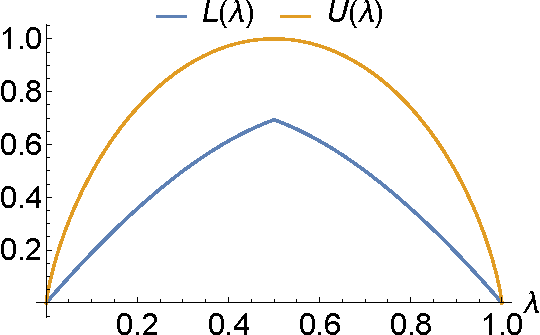
\includegraphics[width=0.5\linewidth]{figures/approximation_ratio.pdf}
		  %  \caption{Caption}
		    \label{fig:approximation-ratio}
		\end{figure}
%		Recall that if $ \lambda=1/2 $, 
%		the generalized Jensen-Shannon divergence reduces to the usual 
%		Jensen-Shannon 
%		divergence. \cref{thm:approximation} yields the approximation 
%		guarantee
%		$
%		0.69< \ln 2 \le \frac{\js{P}{Q}}{H^2(P, Q)} \le 1$.
		
		%\subsection{Hash Family Definition}\label{sub:hash_family}
		
%		If the common sample space $ \Omega $ with which the 
%		two distributions $ P $ and $ Q $ are associated is finite, 
		We  
		identify $ P $ and $Q$ with vectors 
%		the $ |\Omega| $-dimensional vectors 
		$[P(i)]_{i\in 
			\Omega}, [Q(i)]_{i\in \Omega}\in \bR^{|\Omega|} $.
		In this case, 
		$
		H^2(P, Q) = \frac{1}{2} \| \sqrt{P}-\sqrt{Q} \|_2^2$, where $ 
		\sqrt{P} \triangleq [\sqrt{P(i)}]_{i\in \Omega} $ and $ \sqrt{Q} 
		\triangleq 
		[\sqrt{Q(i)}]_{i\in \Omega} $.
%		which is exactly half of the squared $ L^2 $ distance between the two 
%		vectors $ 
%		\sqrt{P} \triangleq [\sqrt{P(i)}]_{i\in \Omega} $ and $ \sqrt{Q} 
%		\triangleq 
%		[\sqrt{Q(i)}]_{i\in \Omega} $. 
		Therefore, the SHD can be 
		endowed with the $ L^2 $-LSH family~\citep{datar2004locality} applied 
		to the 
		square root of the vector. 
		The LSH for the 
		GJSD is 
		\begin{equation}\label{eq:hash_function}
		h_{\mathbf{a}, b}(P) = \left\lceil  \frac{\mathbf{a}^\top \sqrt{P} +b 
		}{r} 
		\right\rceil,
		\end{equation}
		where $ \mathbf{a}\sim \mathcal{N}(0, I) $,
%		 is a $ |\Omega| 
%		$-dimensional standard normal random vector,
%		 $ 
%		\cdot $ denotes the inner product, 
		$ b\sim \operatorname{Unif}[0, r] $,
%		 is uniformly at random on $ [0, r] $,
		  and $ r>0 $.
		
		\structure{\textbf{Theorem~2}}
			Let $ c= \| 
			\sqrt{P}-\sqrt{Q} \|_2$ and $ f_2 $ be the probability density 
			function of the 
			absolute value of $ \cN(0,1) $.	The hash 
			functions $ 
			\{h_{\mathbf{a},b}\}  $ defined in \eqref{eq:hash_function} form a 
			$ (R,c^2\frac{U(\lambda)}{L(\lambda)}R,p_1,p_2) 
			$-sensitive 
			family for the 
			GJSD,
%			 with parameter $ \lambda $, 
			where $ R>0 
			$, $ p_1 = p(1) $, $ p_2=p(c) $, and $
			p(u) = \int_0^r \frac{1}{u}f_2(t/u)(1-t/r)dt$.
		
%		\structure{Triangular Discrimination}
%		Recall that  triangular discrimination is the $ \delta $-divergence, 
%		where $ 
%		\delta(t) = \frac{(t-1)^2}{t+1} $.
%		As shown in the proof of 
%		\cref{thm:lsh_family_triangular_discrimination} 
%		(\cref{sub:proof_triangular_discrimination}), 
%		the function $ \delta $ 
%		can be 
%		approximated by the function $ \hel(t) $ that defines the squared 
%		Hellinger 
%		distance
%		$
%		1\le	\frac{\delta(t)}{\hel(t)} \le 2$.
%		The squared Hellinger distance can be sketched via $ L^2 $-LSH after 
%		taking the 
%		square root, as exemplified in \cref{sub:weighted_js}.
%		By \cref{thm:main}, the LSH family for the square Hellinger distance 
%		also forms 
%		an LSH family for the triangular discrimination.
%		\cref{thm:lsh_family_triangular_discrimination} shows that the LSH 
%		family 
%		defined in  \eqref{eq:hash_function} form a 
%		$ (R,2c^2R,p_1,p_2) 
%		$-sensitive 
%		family for 
%		triangular discrimination.
%		
%		\structure{Theorem }
%			Let $ c= \| 
%			\sqrt{P}-\sqrt{Q} \|_2$ and $ f_2 $ be the probability density 
%			function of 
%			the 
%			absolute value of the standard normal distribution.	The hash 
%			functions $ 
%			\{h_{\mathbf{a},b}\}  $ defined in \eqref{eq:hash_function} form a 
%			$ (R,2c^2R,p_1,p_2) 
%			$-sensitive 
%			family for 
%			triangular discrimination, where $ R>0 
%			$, $ p_1 = p(1) $, $ p_2=p(c) $, and $
%			p(u) = \int_0^r \frac{1}{u}f_2(t/u)(1-t/r)dt$.
		
	\end{block}
	\begin{block}{MIL is a \kr Kernel}
%  		We first show that the MIL is a 
%  		\kr 
%  		kernel. 
 		%\lc{need to review what's \kr kernel in prelim}. 
 		
% 		, 
% 		provided that the associated positive definite kernels allow an 
% 		explicit 
% 		feature map. 
 		
% 		\subsection{Mutual Information Loss is a \kr Kernel}
 		
 		Recall that we assume a joint distribution $ 
 		p(X,C) $.
% 		whose support is $ \cX\times \cC $. 
 		Let $ x,y\in \cX $ be represented 
 		by 
 		$\bfx=[p(c,x):c\in \cC]$, $ \bfy=[p(c,y):c\in 
 		\cC]\in 
 		[0,1]^{|\cC|}$.
 		%  be two vectors, where 
 		%$ x $ and $ y $ are feature values and $ \cC $ denotes the set of all 
 		%possible 
 		%labels. The probability $ p(c,x) $ is the frequency of the data points 
 		%whose 
 		%feature value is $ x $ and whose label is $ c $.
%  		We consider the MIL of merging $ x  $ and $ y $:
%  		$ I(X;C)-I(\pi_{x,y}(X);C)$. 
 		
 		\structure{\textbf{Theorem~4}}
% 			The mutual information loss
 			 $ \mil(\bfx,\bfy) $ is a \kr kernel on 
 			$ 
 			[0,1]^{|\cC|} $: $ \mil=K_1-K_2 $,
% 			 $ \mil(\bfx,\bfy)=K_1(\bfx,\bfy)-K_2(\bfx,\bfy)  $, 
 			 where $ 
 			K_1(\bfx,\bfy) = k(\sum_{c\in \cC}p(c,x), \sum_{c\in \cC}p(c,y)) $ 
 			and
 			 $ 
 			K_2(\bfx,\bfy)=\sum_{c\in \cC} k(p(c,x),p(c,y)) $ are PD kernels, 
 			and
 			$
 			k(a,b) = a\ln\frac{a}{a+b}+b\ln\frac{b}{a+b}
 			$.

 		
% 		To prove \cref{thm:krein_kernel} and
 		To construct explicit feature maps 
 		for $ K_1 $ and $ K_2 $, we need \structure{\textbf{Lemma~3}}.
% 		 the following lemma.
 		
 		\structure{\textbf{Lemma~3}}
 			 $ k $ is a PD kernel on $ [0,1] $ 
 			%  with the  feature map $ x\mapsto \Phi_w(x) $ 
 			s.t.\ 
 			$ k(x,y) = \langle \Phi(x),\Phi(y)\rangle \triangleq \int_\bR \Phi_w(x)^* \Phi_w(y) dw $, 
 			where $
 			\Phi_w(x) \triangleq e^{-iw\ln(x)}
 			\sqrt{x
 			\rho(w)}$, $\rho(w)=\frac{2\sech(\pi 
 			w)}{1+4w^2}$ and $^*$ denotes the complex conjugate.
 			% $ \Phi_w(x)^* $ denotes the complex conjugate of 
 			% $ \Phi_w(x) $.

 		
%  		The map $ \Phi(x):w\mapsto \Phi_w(x) $ is called the \emph{feature map} 
%  		of $ x 
%  		$. 
% 		The integral $ \int_\bR \Phi_w(x)^* \Phi_w(y) dw $ is also denoted 
% 		by a 
% 		Hermitian inner product $ \langle \Phi(x),\Phi(y)\rangle $.
 		
 		%We will show that both kernels $k_1$ and $k_2$ are positive definite 
 		%functions.
 		
% 		\subsection{\kr-LSH for Mutual Information Loss}
 		
% 		Now we are ready to present an asymmetric LSH 
% 		scheme~\cite{shrivastava2014asymmetric} for mutual information 
% 		loss. 
% 		%We would like to remark that 
% 		This method can be easily extended to other \kr kernels, provided that 
% 		the 
% 		associated positive definite kernels admit an explicit feature map.
\end{block}
\end{column} %
\begin{column}{\sepwid}
    
\end{column}
\begin{column}{\onecolwid}
\vspace{-40pt}
    
\begin{block}{Intuition of \kr-LSH: Reduction to Maximum Inner Product Search (MIPS)}
 		We reduce the problem of designing the LSH for a \kr kernel to 
 		the problem of designing the LSH for MIPS~\citep{shrivastava2014asymmetric}.
%  		based on the following intuition.
%  		We call this general reduction \emph{\kr-LSH}.
 		
% 		\subsubsection{Reduction to Maximum Inner Product Search}
 		
% 		Our reduction is based on the following observation.
 		\structure{\textbf{Intuition:}} If 
%  		PD kernels $ K_1 $ and $ K_2$ satisfy
%  		admit 
%  		feature maps $ \Phi_1 $ and $\Phi_2 $ s.t.\
 		$ K_i(x,y)=\langle 
 		\Psi_i(x),\Psi_i(y)\rangle $ ($i=1,2$),
%  		and $ K_2(x,y)=\langle 
%  		\Psi_2(x),\Psi_2(y)\rangle 
%  		$, 
 		then $ K = K_1-K_2 $ can also represented as an inner product 
 		\begin{equation}\label{eq:krein_inner_product}
 		K(x,y)=\langle \Phi_1(x)\oplus \Phi_2(x), \Phi_1(y)\oplus 
 		-\Phi_2(y)\rangle\enspace,
 		\end{equation}
 		where $ \oplus $ denotes the direct sum. 
 		
 		% 		We define $ \rho(w)\triangleq \frac{2\sech(\pi 
% 			w)}{1+4w^2} $. The proposed approach \kr-LSH is presented in 
% 		\cref{alg:krein-lsh}. 
		To make the intuition 
% 		of \eqref{eq:krein_inner_product}
		applicable in a 
		practical implementation, we have
		%The high-level idea is
		to truncate and discretize the 
		integral $ k(x,y) = \int_R \Phi_w(x)^* \Phi_w(y) 
		dw  $. 
% 		First we analyze the truncation. The analysis is similar to 
% 		Lemma~10 of \citep{abdullah2016sketching}.
%  		If we define  $ 
%  		T_1(x) \triangleq \Phi_1(x)\oplus \Phi_2(x)
%  		$ and $ T_2(x)\triangleq \Phi_1(x)\oplus -\Phi_2(x)
%  		$,
%  		then we have $
%  		K(x,y)=\langle T_1(x),T_2(y)\rangle
%  		$.
%  		We call this pair of transforms \emph{left and right \kr transforms}.
		
% 		\begin{algorithm}[tbh]
% 			\caption{ \kr-LSH}\label{alg:krein-lsh}
        
		
% 		We exemplify this technique by applying it to the MIL.

% 		\begin{lemma}[Truncation error bound, proof in 
% 		\cref{app:truncation}]\label{lem:truncation}
% 			If $ t>0 $ and $ x,y\in [0,1] $, the truncation error can be 
% 			bounded as 
% 			follows $
% 			\left| k(x,y) - \int_{-t}^{t} \Phi_w(x)^* \Phi_w(y)  dw \right|  
% 			\le 
% 			4e^{-t}$.
% 		\end{lemma}
% 		To discretize the finite integral $ \int_{-t}^{t} \Phi_w(x)^* 
% 		\Phi_w(y)  dw $, we divide the inteval into $ 2J $ sub-intervals of 
% 		length $ \Delta $. The following lemma bounds the discretization error.
% 		\begin{lemma}[Discretization error bound, proof in 
% 		\cref{app:discretization}]\label{lem:discretization}
% 			If $ J $ is a positive integer, $ \Delta>0 $, and $ 
% 			w_j=(j-1/2)\Delta $, 
% 			the discretization error is bounded as follows $ 
% 			\left| \int_{-\Delta J}^{\Delta J} \Phi_w(x)^* \Phi_w(y)  dw - 
% 			\left\langle \bigoplus_{j=1}^J \tau(x,w_j,j), \bigoplus_{j=1}^J 
% 			\tau(y,w_j,j)\right\rangle\right|
% 			\le 2\Delta
% 			$,
% 			where $ \tau(x,w,j) = 
% 			\left[\cos(w\ln(x))\sqrt{2x\int_{(j-1)\Delta}^{j\Delta} 
% 				\rho(w')dw'},\sin(w\ln(x))\sqrt{ 2x\int_{(j-1)\Delta}^{j\Delta} 
% 				\rho(w')dw' }\right]\in \bR^2 $.
% 		\end{lemma}
		
% 		%Therefore, to guarantee that the error in truncation is at most $ 
% 		%\epsilon $, 
% 		%we require that $ \Delta J \ge \ln(4/\epsilon) $.
% 		%The discretization error is given by 
% 		%\begin{align*}
% 		%&\left| \int_{-\Delta J}^{\Delta J} \Phi_w(x)^* \Phi_w(y)  dw - 
% 		%\sum_{j=1}^{J} 
% 		%2\sqrt{xy}\int_{(j-1)\Delta}^{j\Delta} 
% 		%e^{iw_j\ln(x/y)}\rho(w)dw \right| \\
% 		%\le{} & \sum_{j=1}^{J} 
% 		%2\sqrt{xy}\int_{(j-1)\Delta}^{j\Delta} 
% 		%\left|e^{iw\ln(x/y)}-e^{iw_j\ln(x/y)}\right|\rho(w)dw  
% 		%\le{}  \sum_{j=1}^{J} 
% 		%\sqrt{xy}\int_{(j-1)\Delta}^{j\Delta} 
% 		% \Delta|\ln\frac{x}{y}| \rho(w)dw  \le \Delta\,.
% 		%\end{align*}
% 		%Therefore, if we set $ 
% 		%J=\frac{1+|\cC|}{\epsilon}\ln\frac{4(1+|\cC|)}{\epsilon} 
% 		%$ and $ \Delta = \frac{\epsilon}{1+|\cC|} $, the total approximation 
% 		%loss is at 
% 		%most $ \epsilon $.
		
% 		By \cref{lem:truncation,lem:discretization}, to guarantee that the 
% 		total approximation error (including both truncation and discretization 
% 		errors) is at most $ \epsilon $, it suffices to set $ \Delta = 
% 		\frac{\epsilon}{4(1+|\cC|)} $ and $ J\ge 
% 		\frac{4(1+|\cC|)}{\epsilon}\ln\frac{8(1+|\cC|)}{\epsilon} $.
		
% % 		\subsubsection{LSH for Maximum Inner Product Search}
		
% 		The second stage of our proposed method is to apply LSH to the MIPS 
% 		problem. 
% 		As an example,  
% 		in \cref{ln:simple-lsh}, we use the \splsh introduced by 
% 		\citep{neyshabur2015symmetric}. Let us have a quick review of \splsh. 
% 		Assume 
% 		that $ \cM\subseteq \bR^d $ is a finite set of vectors and that for all 
% 		$ 
% 		\bfx\in \cM $, there is a universal bound on the squared 2-norm, \ie, $ 
% 		\|\bfx 
% 		\|^2_2\le M $.  \citet{neyshabur2015symmetric} assume that $ M=1 $ 
% 		without loss 
% 		of generality. We allow $ M $ to be any positive real number. 
% 		For two vectors $ \bfx,\bfy\in \cM $, \splsh performs the following 
% 		transform $
% 		L_1(\bfx) \triangleq{} 
% 		[\bfx,\sqrt{M-\|\bfx\|^2_2},0], L_2(\bfy) \triangleq{} 
% 		[\bfy,0,\sqrt{M-\|\bfy\|^2_2}]$.
% 		Note that the norm of $ L_1 $ and $ L_2 $ is $ M $ and that therefore 
% 		their cosine similarity equals their inner product. 
% 		In fact, \splsh is a reduction from MIPS to LSH for the cosine 
% 		similarity. Then a random-projection-based LSH for the cosine 
% 		similarity~\citep{charikar2002similarity,wang2014hashing} \[ 
% 		h(\bfx)\triangleq \sign(\bfx^\top L_i(\bfx)),\quad \bfa\sim \cN(0, I), 
% 		i=1,2
% 		\]
% 		can be used for MIPS and thereby LSH for the MIL divergence via our 
% 		reduction.
% 		% By Theorem~4.2 of 
% 		%\citep{neyshabur2015symmetric}, we know that \kr-LSH is a $ 
% 		%(S,cS,p_1,p_2) 
% 		%$-LSH for any $ 0<S<1 $ and $ 0<c<1 $.
		
% 		%Let $ K(\bfx,\bfy) = k_1(\bfx,\bfy)-k_2(\bfx,\bfy)$ be a \kr kernel, 
% 		%where $ 
% 		%k_1 $ and $ k_2 $ are two positive definite kernels.
		
% % 		\paragraph{Discussion}
% 		We have some important remarks for practical implementation of \kr-LSH. 
% 		Although \citep{neyshabur2015symmetric} provides a theoretical 
% 		guarantee for 
% 		LSH for MIPS, as noted in~\citep{yan2018norm}, the additional term $ 
% 		\sqrt{M-\|\bfx\|_2^2} $ may dominate in the $ 2 $-norm and 
% 		significantly 
% 		degrade the performance of LSH. To circumvent this issue, we recommend 
% 		a method 
% 		that partitions the dataset according to the $ 2 $-norm, \eg, the 
% 		norm-ranging 
% 		method~\citep{yan2018norm}.
	\end{block}
	\begin{block}{Algorithm \kr-LSH}
			\begin{algorithmic}[1]
				\Require Discretization parameters $ J\in \mathbb{N} $ and $ 
				\Delta>0 $.
				\Ensure The left and right \kr transform $ \eta_1 $ and $ 
				\eta_2 $.
				\State $ w_j \gets (j-1/2)\Delta $ for $ j=1,\dots,J $
				%\State Sample $w_1,\dots,w_L,w'_1,\dots,w'_{L'}$ i.i.d.\ from 
				%the 
				%distribution 
				%with density \[\frac{\sech(\pi w)}{\ln(2)(1+4w^2)}\,.\]
				\State Construct the atomic transform \begin{align*}
				\tau(x,w,j)\triangleq{}&
				\left[\cos(w\ln(x))\sqrt{2x\int_{(j-1)\Delta}^{j\Delta} 
					\rho(w')dw'},\right.\\
					& \left.\sin(w\ln(x))\sqrt{ 
					2x\int_{(j-1)\Delta}^{j\Delta} 
					\rho(w')dw' }\right]
				\,.
				\end{align*}
				\State Construct the left and right basic transform 
				\begin{align*}
				\eta_1(\bfx)\triangleq{} & \bigoplus_{j=1}^J 
				\tau(p(x),w_j,j)\oplus 
				\bigoplus_{j=1}^{J} \bigoplus_{c\in \cC} \tau(p(c,x),w_j,j)\,,\\
				\eta_2(\bfx)\triangleq{} & \bigoplus_{j=1}^J 
				\tau(p(x),w_j,j)\oplus 
				\bigoplus_{j=1}^{J} \bigoplus_{c\in \cC} -\tau(p(c,x),w_j,j)\,.
				%\eta_2(\bfy,\bfw,\bfw',L,L')\triangleq{} & \bigoplus_{j=1}^L 
				%\tau(p(y),w_j,L)\oplus \bigoplus_{j=1}^{L'} \bigoplus_{c\in 
				%\cC} 
				%-\tau(p(c,y),w'_j,L')\,.
				\end{align*}
				%\State \Return $ \eta_1 $ and $ \eta_2 $
				\State Construct the left and right \kr transform
				\begin{align*}
				T_1(\bfx,M) \triangleq{} & 
				[\eta_1,\sqrt{M-\|\eta_1(\bfx)\|^2_2},0],\\ T_2(\bfy,M) 
				\triangleq{} &
				[\eta_2,0,\sqrt{M-\|\eta_2(\bfx)\|^2_2}]\,.
				\end{align*}
				where $ M $ is a constant such that $ M\ge \|\eta_1(\bfx)\|_2^2 
				$ (note 
				that $ 
				\|\eta_1(\bfx)\|_2 = \|\eta_2(\bfx)\|_2 $).
				\State Sample $\bfa\sim \cN(0,I)$ and construct the hash 
				function 
				$ h(\bfx; M)\triangleq \sign(\bfa^\top T(\bfx, M))$,
				where $T$ is either the left or right 
				transform.\label{ln:simple-lsh}
				%\State Rank the feature values $ \bfx $ in the vocabulary $ 
				%\cM $ 
				%according to 
				%$ \|\eta_1(\bfx)\|_2 $.
				%\State Partition the vocabulary of feature values $ \cM $ into 
				%$ m $ 
				%sub-vocabularies $ \{ \cM_1,\dots,\cM_m \} $ such that the 
				%sub-vocabulary $ 
				%\cM_i 
				%$ contains the feature values whose $ \|\eta_1(\bfx)\|_2 $ are 
				%ranked 
				%in the 
				%range $ [(i-1)\frac{|\cM|}{m},i\frac{|\cM|}{m}] $.
				%\For{each sub-vocabulary $ \cM_i $}
				%\State Build 
				%\EndFor
			\end{algorithmic}
% 		\end{algorithm}
        \end{block}
\end{column}
 
		
	\end{columns} %
	
\end{frame} %

\end{document}